\documentclass{article}

\usepackage{graphicx}
\usepackage{subcaption}
\usepackage{amsmath}
\usepackage{float}
\usepackage{listings}
\usepackage{xcolor}
\usepackage{float}

\lstset{
    language=Java,
    basicstyle=\ttfamily\footnotesize,
    breaklines=true,
    numbers=left,
    stepnumber=1,
    numbersep=5pt,
    showspaces=false,
    showstringspaces=false,
    tabsize=2
}

\title{Sistemas Distribuídos - Atividade 1: Serialização}
\author{André Filipe de Medeiros - 542104}
\date{\today}

\begin{document}
\maketitle

\newpage
\section{Resumo}
A presente atividade visa avaliar o impacto de diferentes protocolos de serialização no tamanho de mensagens trocadas entre processos (cliente e servidor) em Java. Analizaram-se cinco tipos de serialização: padrão do Java (com e sem customização), JSON, XML e Protobuf, em dois cenários: um com baixo volume de dados (requisição de compra) e outro com maior volume (agenda de contatos). Com auxílio do Wireshark, comparou-se o número de bytes enviados em cada contexto.
 Por fim, a serialização pelo protocolo Protobuf aparenta ser uma boa opção, pois apresentou eficiência em termos de compactação e pode ser utilizado em diferentes sistemas.

\section{Discussão Técnica}

\subsection{Serialização}
A serialização é um procedimento responsável por transformar um objeto ou estrutura de dados em um formato possível de ser armazenado ou transmitido. Nesse sentido, a serialização é fundamental para que sistemas diferentes se comuniquem no contexto de computação distribuída.

Atualmente, existem diferentes protocolos que implementam a serialização como a serialização padrão do Java, serialização customizada do Java, JSON, XML e Protobuf. 

\section{Metodologia}

\subsection{Código}
Os códigos foram escritos na linguagem Java. Programou-se dois programas para cada protocolo e cenário. O primeiro programa é referente ao processo servidor, que foi executado no endereço \textit{localhost} e porta $6789$. O papel do processo servidor é de apenas receber a mensagem do processo cliente e imprimir a mensagem no terminal. Enquanto, no processo cliente, instanciam-se objetos e os enviam ao processo servidor. 

Ao todo, criaram-se códigos a dez cenários:
\begin{equation}
    N = 5 \;(prot.\, de \,serializacao) \times 2 \;(compra\, e\, agenda) = 10
\end{equation}
Os códigos estão disponíveis em: {https://github.com/andredemedeiros/serializations.git}

\subsection{Captura de pacotes}
A captura de pacotes ocorreu em três etapas. A primeira etapa foi referente a inicialização de captura de pacotes através do Wireshark. Na segunda etapa, executaram-se os processos servidor e cliente, respectivamente, para que os objetos fossem serializados e transmitidos. 
Por fim, os dados da captura foram salvos em formato \textit{.pcap} e estão disponíveis no repositório. 

\begin{figure}[H]
    \centering
    \caption{Captura de pacotes da serialização padrão no cenário de requisição de compra.}
    \begin{subfigure}[b]{0.7\textwidth}
        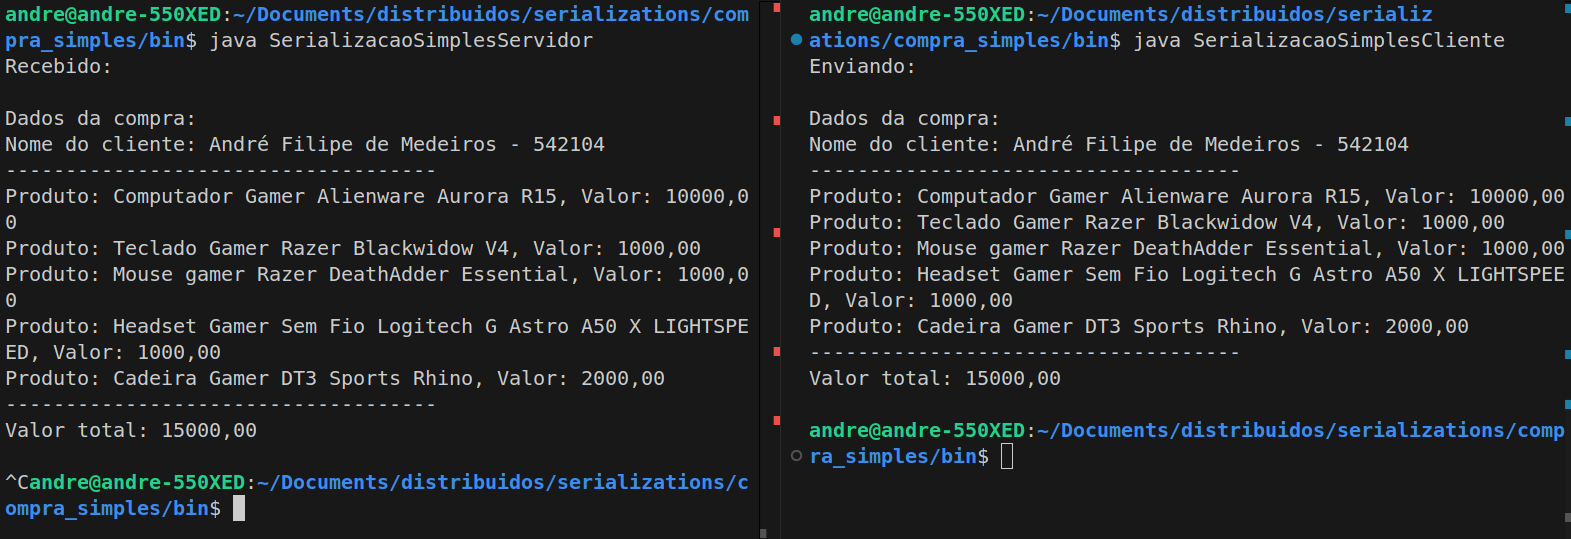
\includegraphics[width=\textwidth]{imgs/compra_simples_term.png}
        \caption{Execução dos processos servidor e cliente com protocolo de serialização padrão do Java.}
        \label{fig:clock_original}
    \end{subfigure}%

    \begin{subfigure}[b]{0.7\textwidth}
        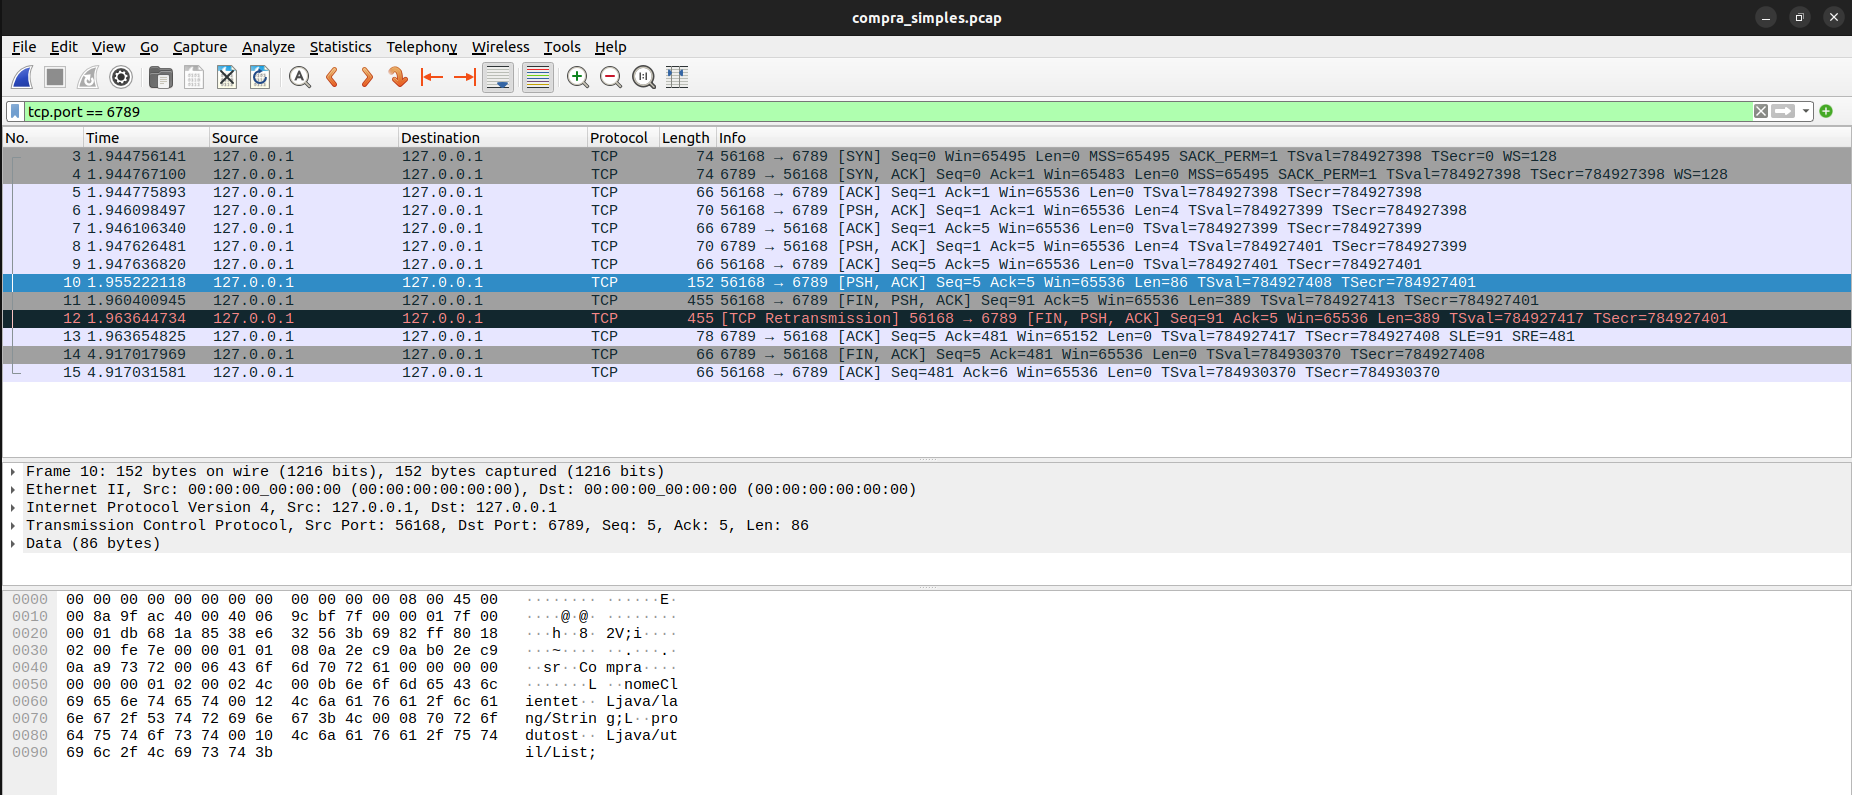
\includegraphics[width=\textwidth]{imgs/compra_simples_wire.png}
        \caption{Captura dos pacotes trocados pelos processos cliente e servidor com protocolo de serialização padrão do Java.}
        \label{fig:clock_300dpi}
    \end{subfigure}%
    \label{fig:clock_comparison}
\end{figure}

Aplicou-se o mesmo procedimento de captura de pacotes em todos cenários.

\subsection{Cálculo de tamanho de pacotes}
Os pacotes do cenário que simula uma requisição de compra, possui um volume considerávelmente menor em comparação com os
pacotes do cenário que simula uma agenda de contatos. Por isso, no primeiro cenário, foi possível calcular manualmente (com arquivos os \textit{.pcap}) a quantidade de \textit{bytes} necessária para transmitir a mensagem após serialização. No seguindo caso, porém, utilizou-se o \textit{sotware} \textit{tshark} que automatiza a leitura e operação em arquivos \textit{.pcap}.



\section{Discussão dos Resultados}

Após a escrita dos \textit{scripts} em Java que implementam a serialização e de posse dos arquivos \textit{.pcap} com os tamanhos dos pacotes transmitidos (em \textit{bytes}) foi possível
gerar gráficos de barras comparativos entre os protocolos em diferentes cenários.

\begin{figure}[H]
    \centering
    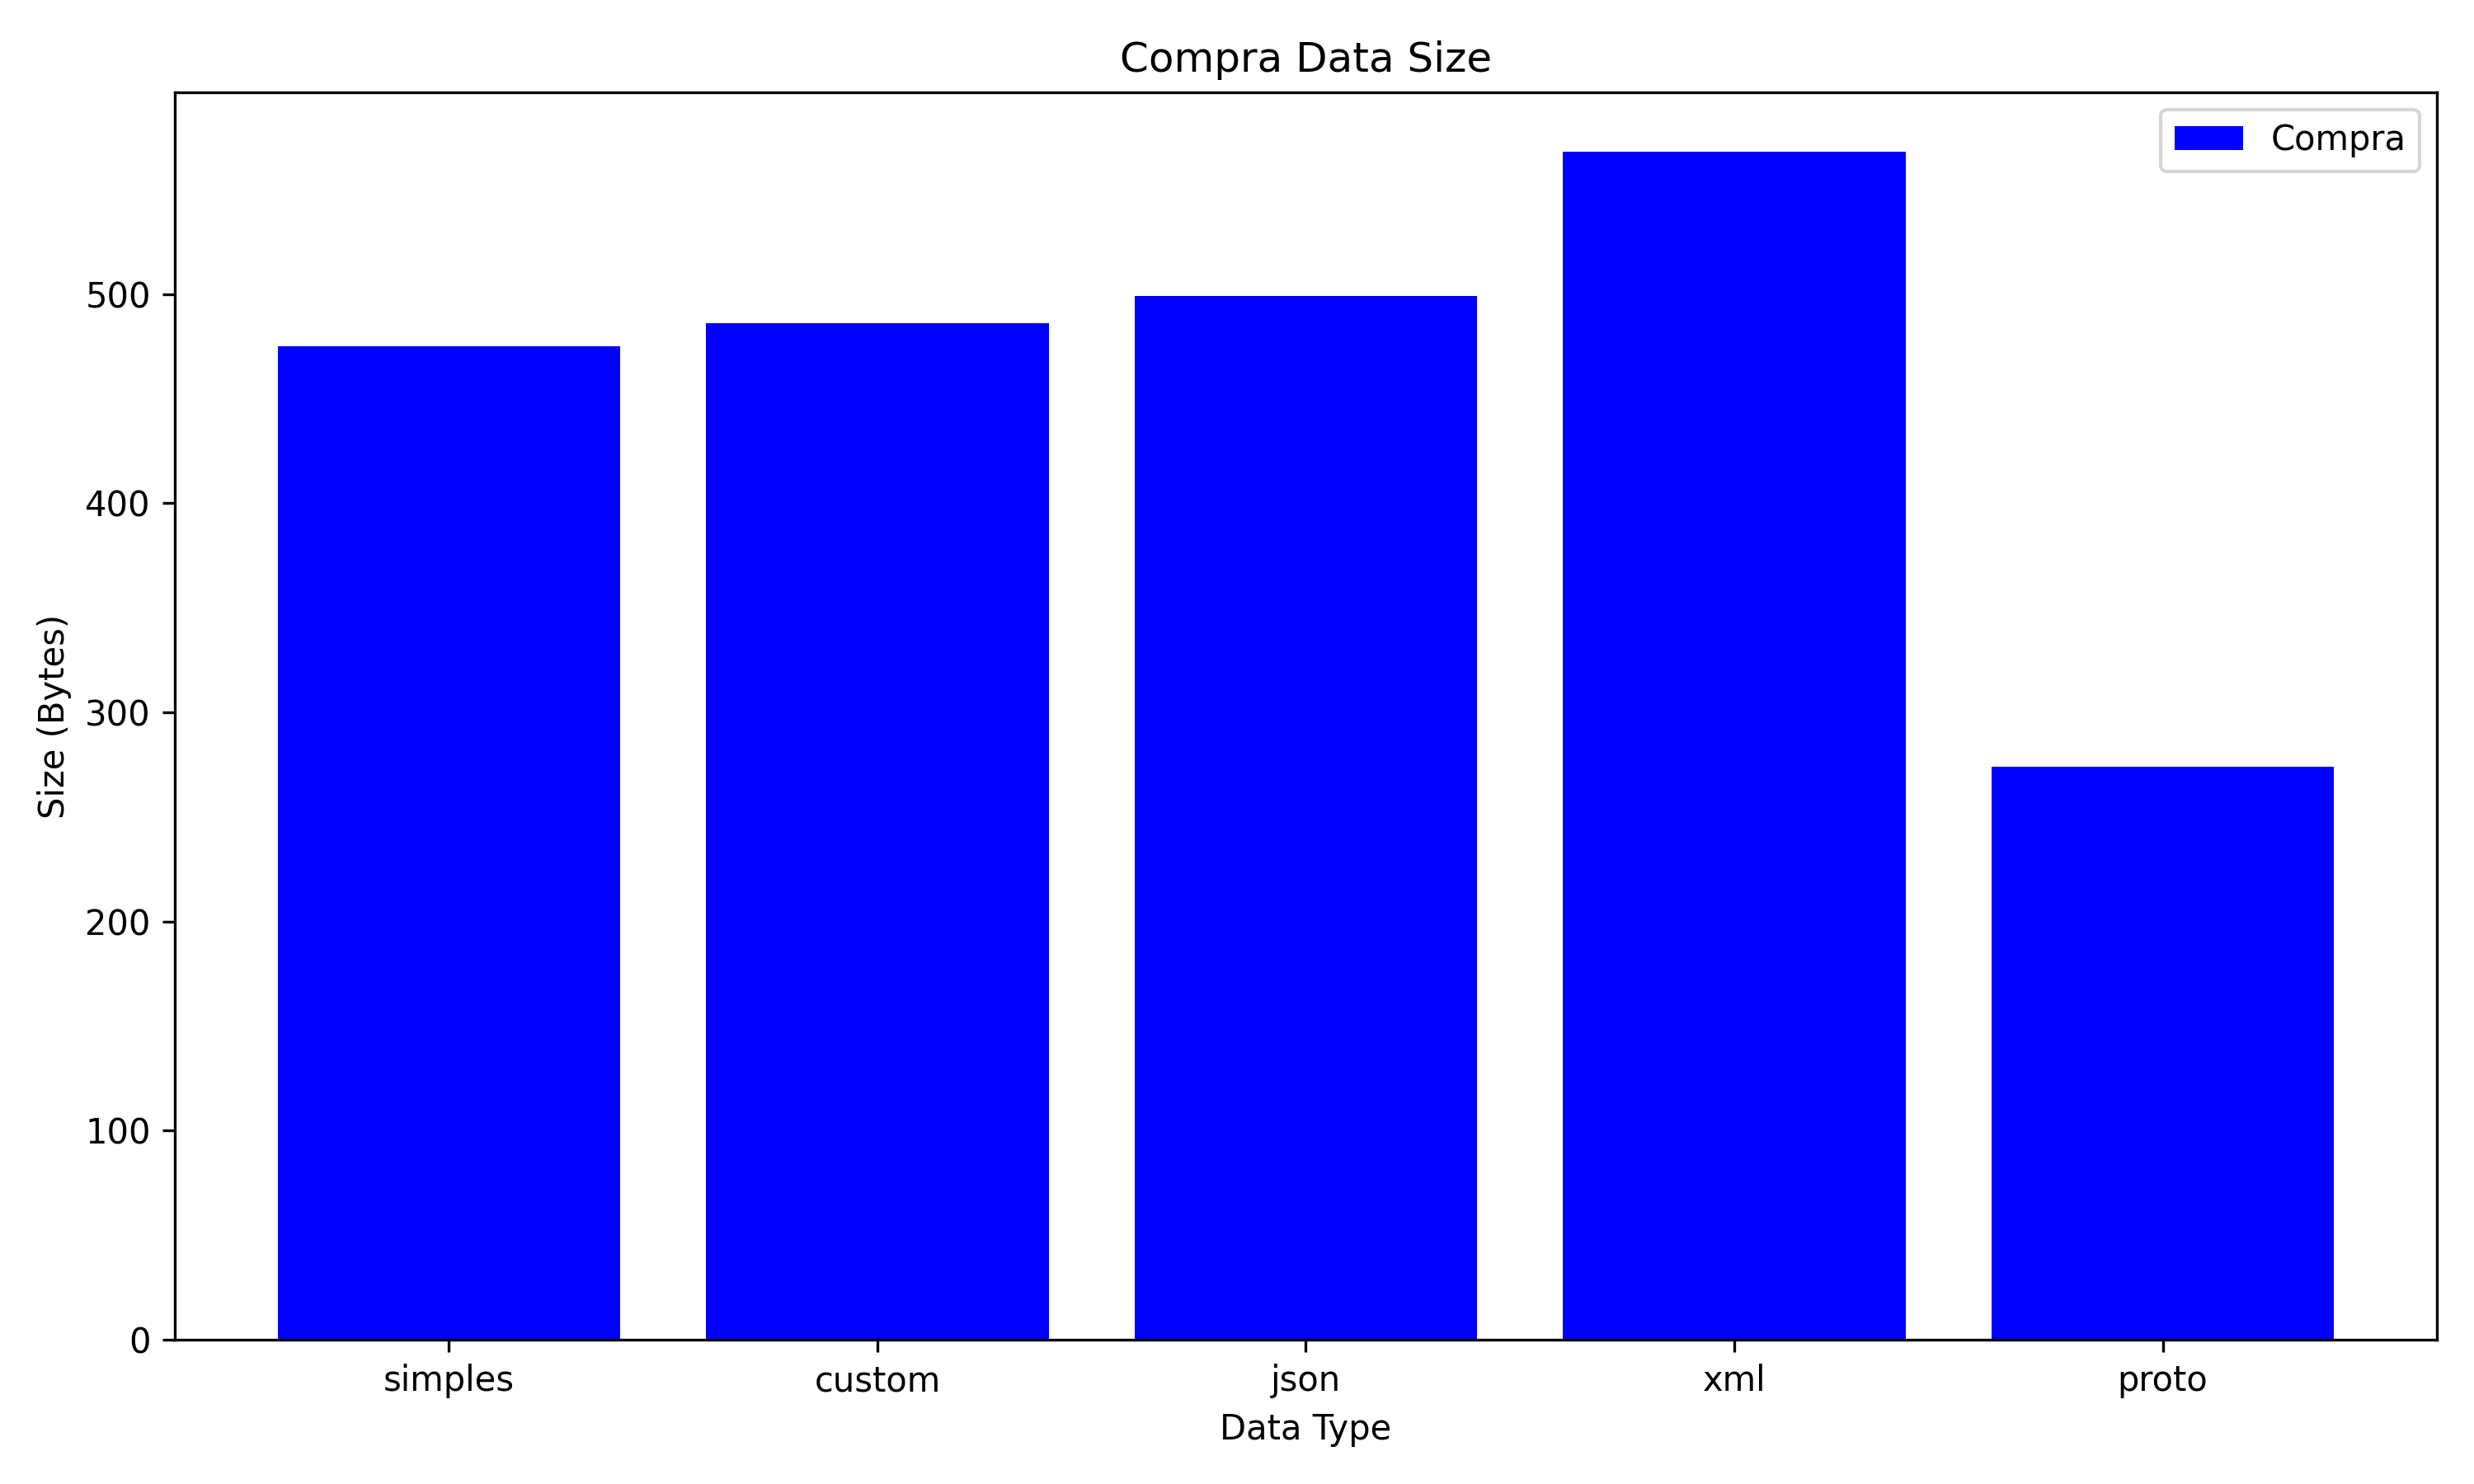
\includegraphics[width=\textwidth]{imgs/compra_data_size.png}
    \caption{Tamanho das mensagens enviadas após serialização, cenário de requisição de compra.}
    \label{fig:compra}
\end{figure}

Observa-se pela Figura \ref{fig:compra} que o protocolo de serialização Protobuf apresenta uma eficiência considerável em termos de compactação, quando comparado aos outros protocolos.

\begin{figure}[H]
    \centering
    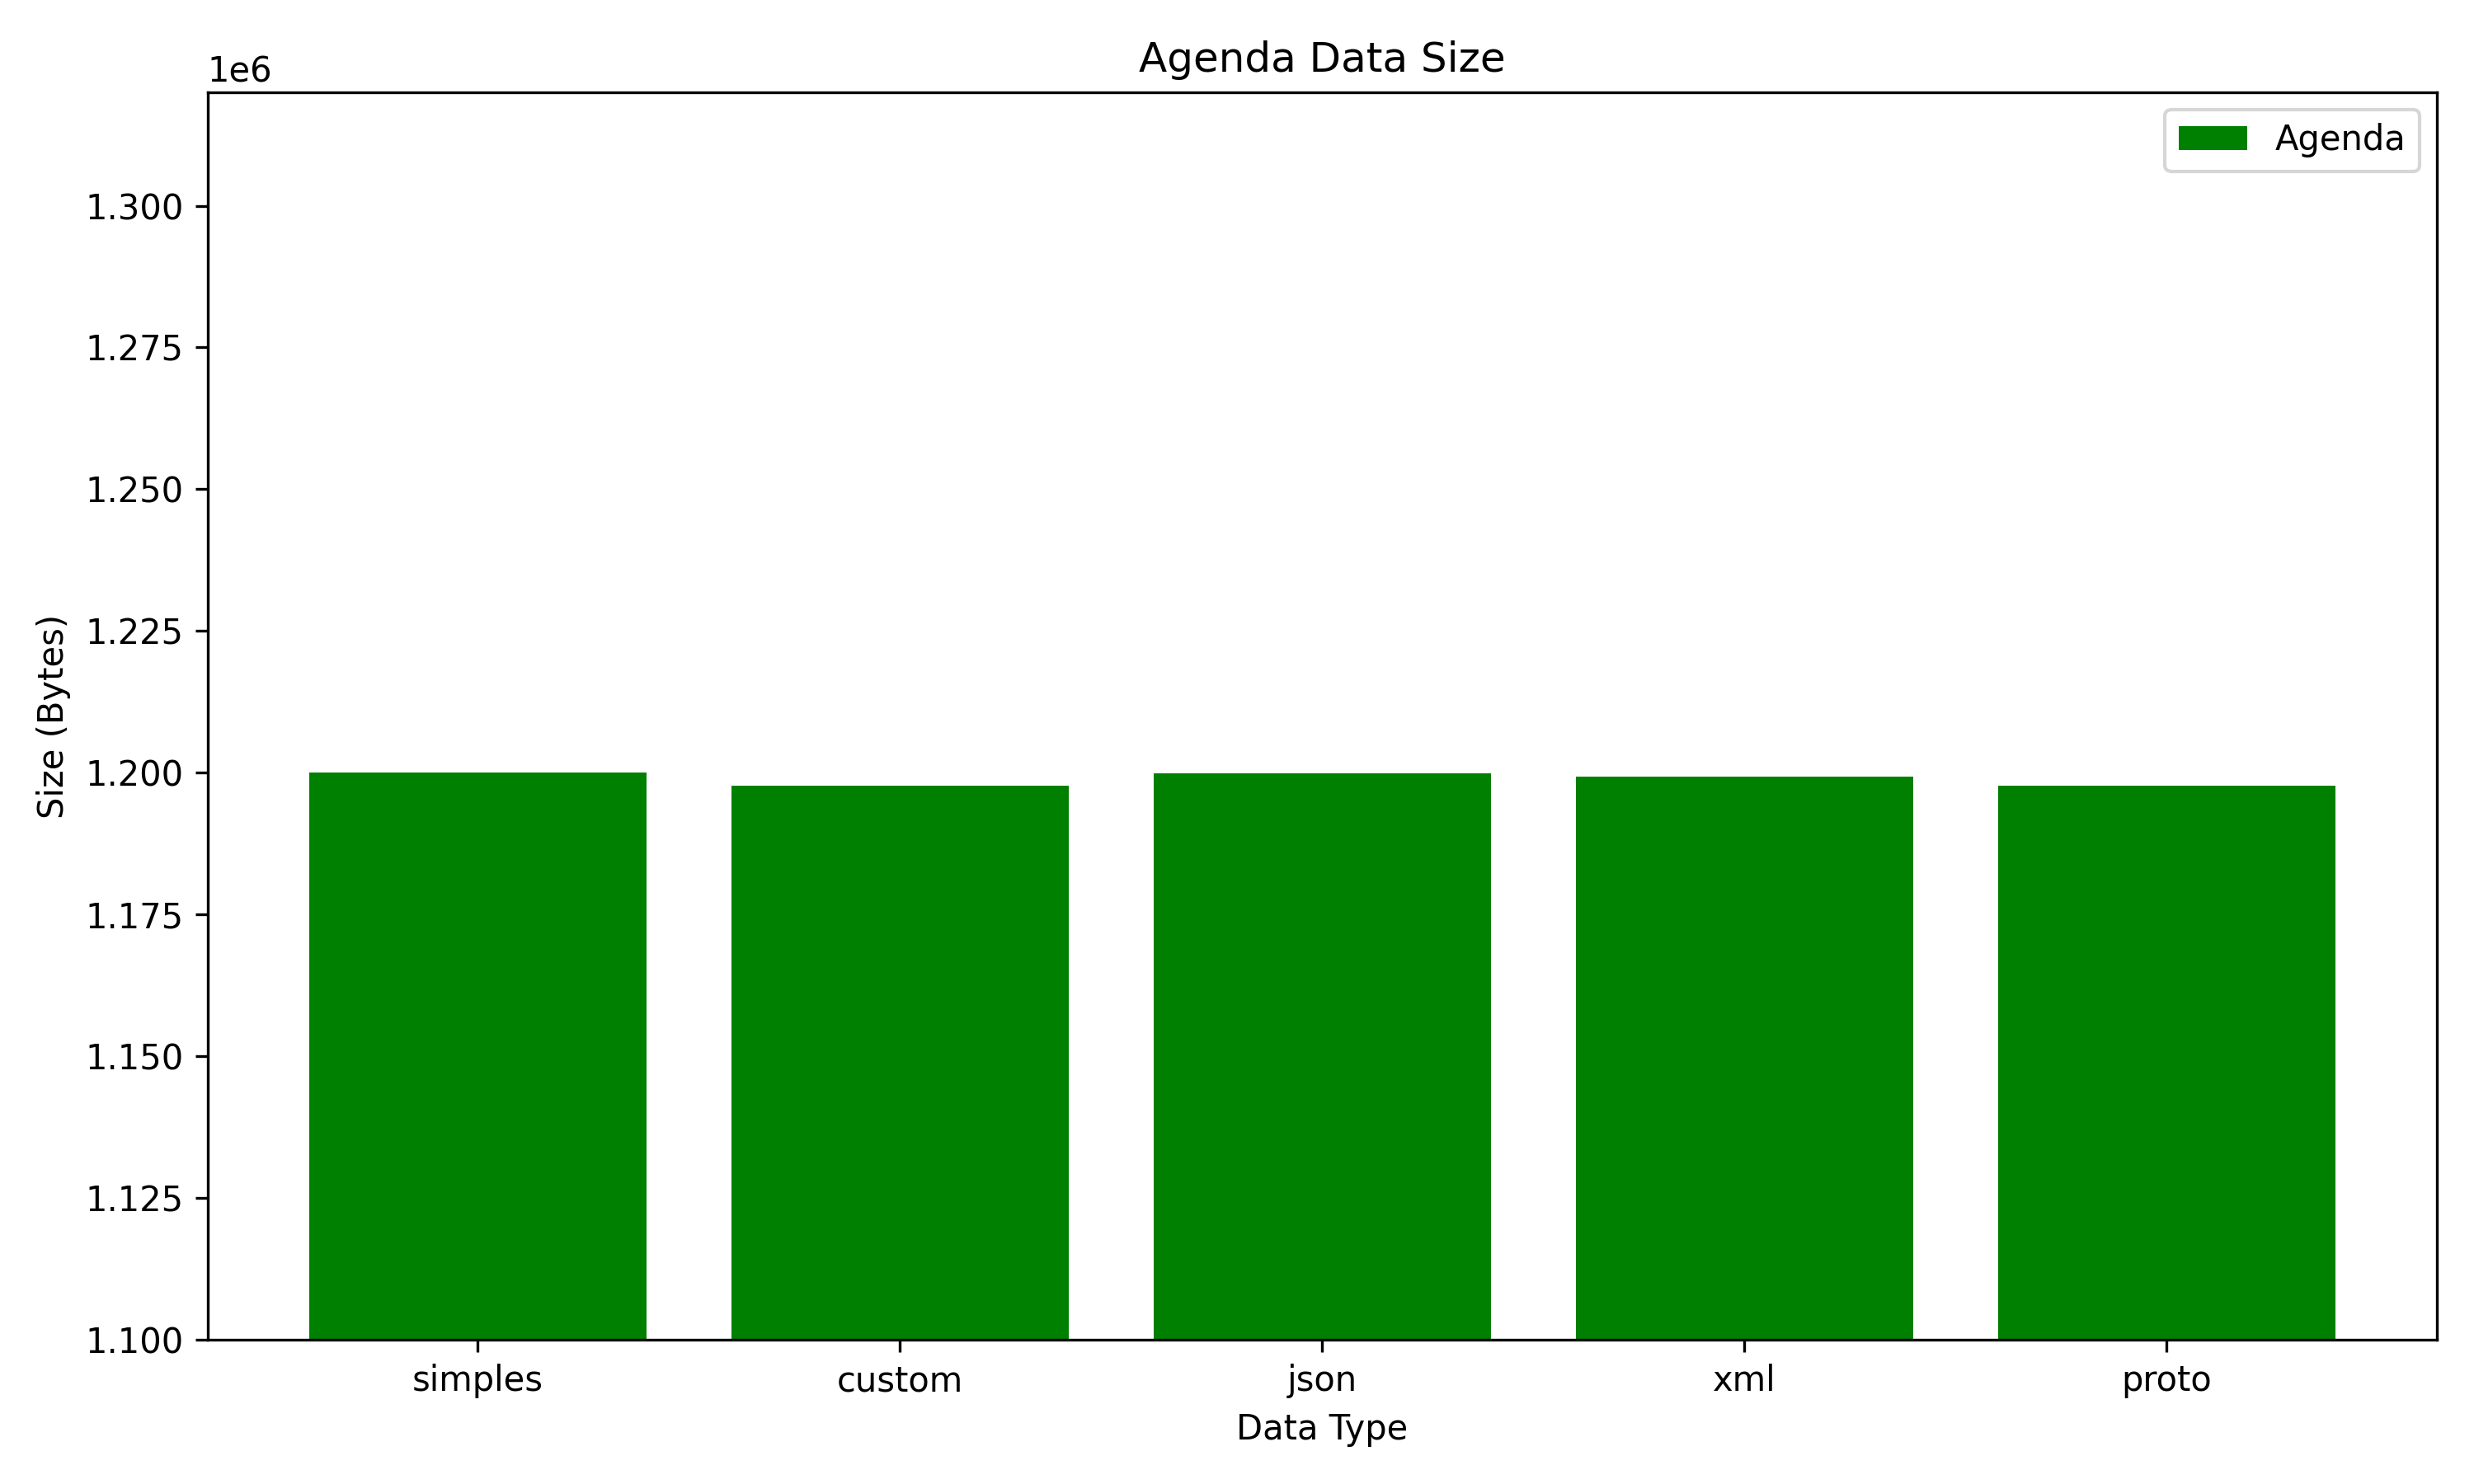
\includegraphics[width=\textwidth]{imgs/agenda_data_size.png}
    \caption{Tamanho das mensagens enviadas após serialização, cenário de agenda de contatos.}
    \label{fig:agenda}
\end{figure}

No segunda caso, Figura \ref{fig:agenda}, porém, percebe-se que para mensagens que possuem imagens a discrepância percentual entre a eficiência dos protocolo de serialização é menor. O melhor protocolo de serialização nesse caso foi o customizado. Mesmo assim, o protocolo Protobuf também apresentou uma boa eficiência em comparação aos outros protocolos.

\begin{table}[ht]
    \centering
    \begin{tabular}{l|r|r|r|r}
    \hline
    \textbf{Categoria} & \multicolumn{2}{c|}{\textbf{Compra}} & \multicolumn{2}{c|}{\textbf{Agenda}} \\
    \hline
    & \textbf{Valor (B)} & \textbf{+/- Média (\%)} & \textbf{Valor (B)} & \textbf{+/- Média (\%)} \\
    \hline
    \textbf{Padrão}   & 475   & -3.5\%  & 1,199,998  & 0.07\%  \\
    \textbf{Custom}   & 486   & 5.6\%   & 1,197,660  & -0.12\% \\
    \textbf{JSON}     & 499   & 8.4\%   & 1,199,956  & 0.07\%  \\
    \textbf{XML}      & 568   & 23.3\%  & 1,199,362  & -0.06\% \\
    \textbf{Protobuf} & 274   & -40.5\% & 1,197,724  & -0.11\% \\
    \hline
    \end{tabular}
    \caption{Tabela de Dados de Compra e Agenda com Valores e Comparativo Percentual}
    \label{tabela}
\end{table}

A Tabela \ref{tabela} apresenta um comparativo resumido entre os protocolos de serialização em diferentes cenários. Além disso, pode-se comparar, em cada cenário, o percentual de eficiência de um protocolo utilizado em relação à média. 

\vbox{} Conclui-se que os protocolos de serialização resultam em diferentes eficiências de compactação. Essas diferenças estão relacionadas ao protocolo e à maneria que a serialização foi implementada. Além disso, o melhor protocolo de serialização varia de sistema para sistema. No cenário de lista de compras, o Protobuf foi considerávelmente eficiente. Porém, no cenário de 
agenda de contatos, a serialização customizada foi mais eficiente. No entanto, em ambos casos, o Protobuf foi o único protocolo que apresentou eficiência maior que a média. Além disso, esse protocolo pode ser implementado em sistemas além do Java.

\end{document}